\documentclass[bachelor]{njupthesis}

\title{这是标题}
\author{这是你的名字}
\advisor{导师的名字}
\school{某某学院}
\major{某某专业}
\studentclass{Q/B17xxxx}
\studentid{Q/B17xxxxxx}
\graduateyear{2021}
\begindate{202x年3月x日}
\finishdate{202x年x月x日}


\begin{document}

\makecover

\begin{chineseabstract}
南京南站(Nanjingnan Railway Station)位于江苏省南京市雨花台区,是中国铁路上海局集团有限公司管辖的客运站,是南京铁路枢纽的重要组成部分,也是华东地区最大的交通枢纽 ,国家铁道枢纽站 ,是亚洲第一大火车站。
南京南站规划于1986年,地处南京南部新城的核心区;1991年进入早期规划阶段;2008年1月正式开工,北靠雨花台风景区、南临秦淮新河、西接牛首山;2008年8月规划设计方案最终确定;2011年6月28日南京南站及北广场正式投入使用,成为中国第一个通过垂直换乘实现真正零换乘的交通枢纽,其“垂直换乘”的设计理念被铁道部全面推广和使用。 
截至2019年12月,南京南站占地面积约70万平方米,总建筑面积73万平方米,站房总建筑面积约45.8万平方米,其中主站房面积达38.7万平方米,是亚洲最大的火车站,总投资超过300亿元人民币,站房建筑秉承“古都新站”的设计理念,吸纳了大量中国古典建筑元素,如藻井、斗拱、窗花和木纹肌理等,同时中西合璧、兼收并蓄,将中国宫殿建筑的优势及特点充分发挥,体现了古都南京浓郁的风格和特有的气质。


\chinesekeyword{南京南站;铁道部;京沪高铁;南京}
\end{chineseabstract}

\begin{englishabstract}
Nanjingnan Railway Station is located in Yuhuatai District, Nanjing city, Jiangsu Province. It is a passenger Station under the jurisdiction of China Railway Shanghai Group Co., LTD. It is an important part of Nanjing Railway Hub, the largest transportation hub in East China, the national Railway hub Station, and the largest Railway Station in Asia.
Planned in 1986, Nanjing South Railway Station is located in the core area of the new city in the south of Nanjing. It entered the early planning stage in 1991; Construction started in January 2008, with Yuhuatai Scenic Spot in the north, Qinhuai New River in the south and Niushou Mountain in the west. In August 2008, the planning and design scheme was finalized; On June 28, 2011, Nanjing South Railway Station and North Plaza were officially put into use, becoming the first transportation hub in China to realize real zero transfer through vertical transfer. Its design concept of "vertical transfer" was fully promoted and used by the Ministry of Railways.
As of December 2019, the nanjing south railway station area of about 700000 square meters, a total construction area of 730000 square meters, the station building a total construction area of 458000 square meters, of which the main room area of 387000 square meters, is Asia's largest railway station, with a total investment of more than 30 billion yuan, the station building adhering to the "ancient capital of xinzhan" design concept, Absorbing a large number of Chinese classical architectural elements, such as sunk panels, brackets, window cuts and wood texture, etc., the combination of Chinese and Western elements, eclectic, gives full play to the advantages and characteristics of Chinese palace architecture, reflecting the rich style and unique temperament of the ancient capital Nanjing.

\englishkeyword{Nanjing South Railway Station;xx;B站;Nanjing}
\end{englishabstract}

\thesistableofcontents

\thesischapterexordium

\chapter{绪论}
1986年,南京市整体规划向南发展,决定在主城南部建设大型车站,并预留了南京南站地区的规划空间。
1990年12月,原中华人民共和国铁道部完成《京沪高速铁路线路方案构想报告》。京沪高铁的前期工作进展,极为缓慢,甚至搁浅停滞相当长的一段时间,铁路要在速度上与民航竞争很多人持怀疑态度。
1991年,南京南站进入早期规划阶段。

\section{名字自己替换}
\subsection{名字自己替换}
1994年12月,中国国务院批准开展京沪高速铁路预可行性研究。铁道部开展京沪高铁选线,提出“北线方案”,即从上元门地区,通过隧道过江。南京的规划部门则拿出“南线方案”,从大胜关过江。铁道部牵头,进行比选得出的结论是:两个方案在技术上都可行,主要差别在于工程造价、经济效益、运营条件等方面。江苏省和南京市要求南线方案,而铁道部看好的始终是北线方案。南京力主南线,是放长了眼光。如果从南京北部走,已经不具备扩建条件。南京火车站虽然前面是玄武湖、背面是小红山,景观很美,但是已经没有拓展空间。此外,更重要的是,在全国任何一个城市,铁路带动城市发展的效果都非常明显,南京要想进一步发展南部区域,这是个好机会。显然,高铁建在哪里,也就意味着南京今后的发展框架,是继续囿于老城狭小的空间里,还是大步向南拓展。铁道部青睐北线的理由:新线与既有线的衔接方便。清末修建的津浦铁路,即从天津到浦口;在长江南岸,之后又修建了沪宁铁路。浦口火车站、下关火车站、南京站,南京重要的火车站,向来都是位于城北。并且,当时铁道部的人都认为,南京的城市中心就在北边。另一方面,铁路的机务段、职工宿舍等都在城北,建成之后,职工上下班都方便。为了说服铁道部,南京方面列出了南线的九大优势:无论高铁从哪里走,从完善南京枢纽总体布局的角度来看,都必须建大胜关长江大桥;根据国务院批准的南京城市规划,南京城市今后将主要向东南方向发展,大胜关方案符合城市扩展方向;南面的场站位置已预留多年,有较为理想的建站条件;沿线拆迁量小,对城市干扰和环境影响小;利于形成方便的铁路——航空换乘及铁路与城市道路联结条件……不过,这些最初并没有打动铁道部,铁道部仍然坚持北线方,双方为此对峙了好几年。


\subsection{名字自己替换}
1995年,为了促进高铁尽快上马,南京稍稍“松口”。在当年的一份紧急报告里,有这样一句话——“南北方案之争不宜过多坚持,而从规划上对北线方案提出完善意见为妥”。南京市规划局做了两手准备,针对南线、北线方案,分别做了规划控制。从1995年起,南京根据两个方案,开始分别严格控制沿线用地建设,同时冻结了南北两条线周围的土地。而这个具有预见性的做法,使得后来的工作变得轻松许多。

南京南站如图\ref{南京南站}所示。
\begin{figure}[hbt]
	\centering
	\subfigure[南京南1]{
		\begin{minipage}[b]{0.4\textwidth}
			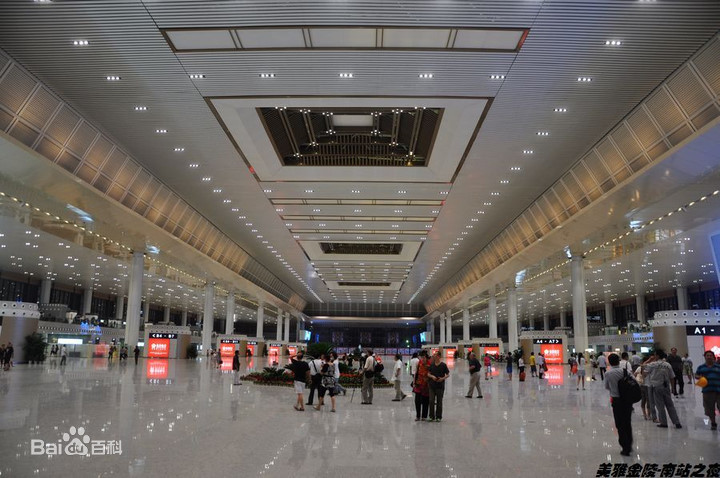
\includegraphics[width=1\textwidth]{1}
		\end{minipage}
	}
	\subfigure[南京南2]{
		\begin{minipage}[b]{0.4\textwidth}
			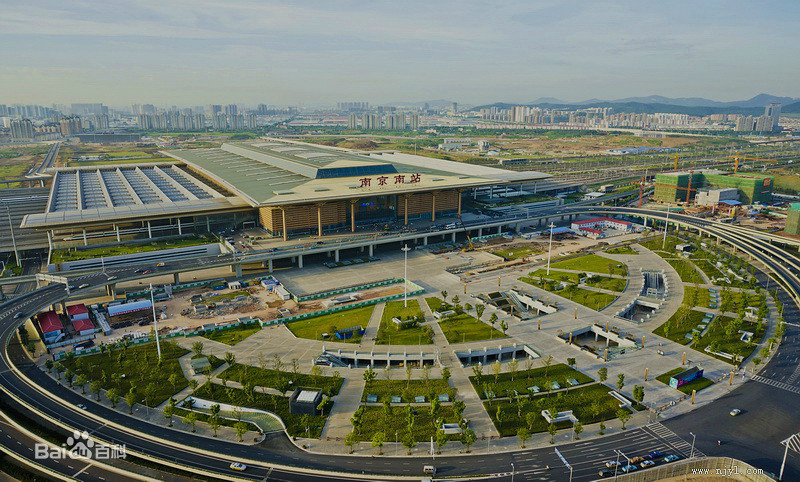
\includegraphics[width=1\textwidth]{2}
			
		\end{minipage}
	} \\
	\subfigure[南京南3]{
		\begin{minipage}[b]{0.4\textwidth}
			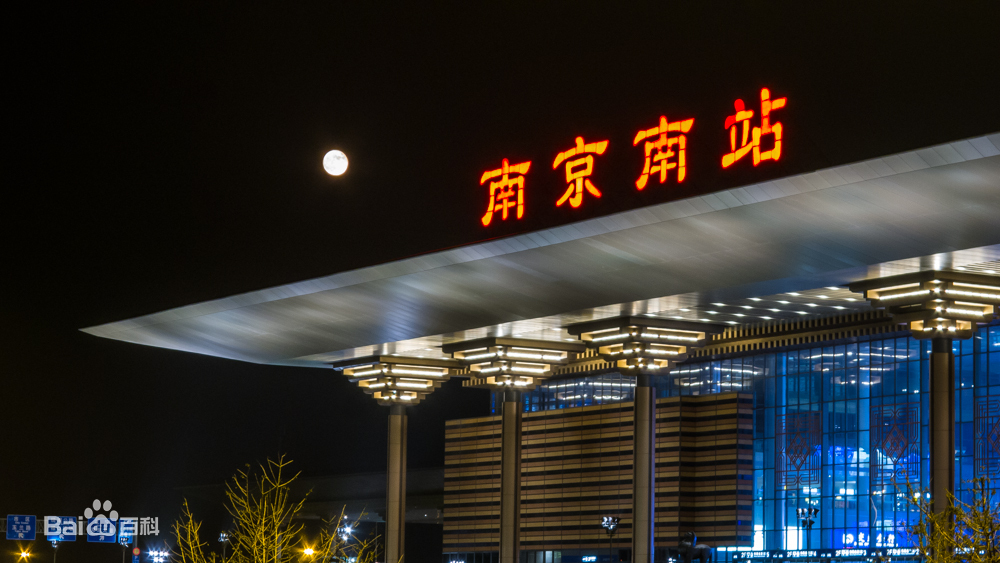
\includegraphics[width=1\textwidth]{3}
		\end{minipage}
	}
	\subfigure[南京南4]{
		\begin{minipage}[b]{0.4\textwidth}
			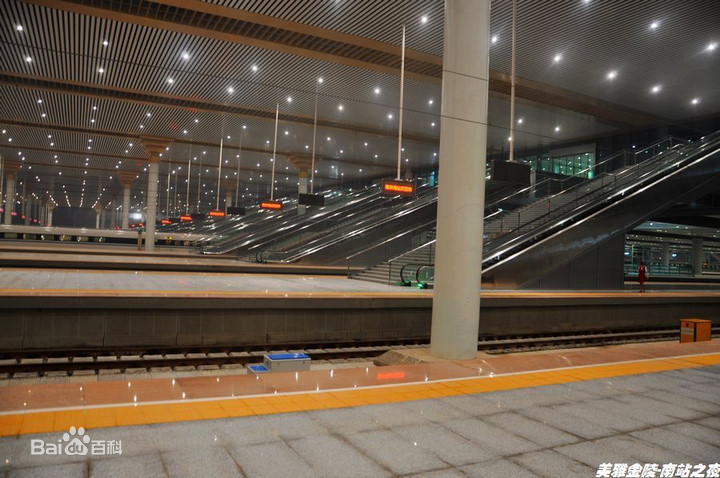
\includegraphics[width=1\textwidth]{4}
			
		\end{minipage}
	}
	\caption{南京南站}
	\label{南京南站}
\end{figure}


\section{俄罗斯和乌克兰}
本论文主要创新点与贡献如下\cite{荣洁2005俄罗斯民族性格和文化}:

xxxxxxxxxxxxxx


\section{什么是快乐星球}
本文的章节结构安排如下:

xxxxxxx
%Another possible solution is using a dynamic strategy to adaptively switch between the exploration phase and the exploitation phase. 
%As the explored paths increase, the exploitation phase is gradually invoked, in which high-valued directed seeds are selected and prioritized to enhance the reachability. When the fuzzer can not find any new paths for a long while, the exploration phase has come to a bottleneck and should move to the exploitation phase. Similarly, there are occasions that should move from the exploitation phase back to the exploration phase. For example, when the exploitation phase cannot get any closer to the target for many fuzzing cycles, it should step back to the exploration phase. This is because the directed seeds in hand perform poorly, and we should enlarge path coverage to discover more potential directed seeds. With this scheme, both of the two phases can coexist to achieve the best performance and adaptiveness. 



\begin{table}[t]
\vspace{2ex}
\centering
\small 
\begin{tabular}{p{8.4cm}}
\hline
 
Algorithm 2: DGF with adaptive splitting of exploration and exploitation. \\   
\hline
01 $seedQ \leftarrow i$ \quad /* initial seeds*/ \\
02 $dp \leftarrow 0$ \\
03 $directedQ \leftarrow \varnothing$ \quad /* Queue for directed seeds */\\
04 $noPathCycles \leftarrow 0$ \\
05 $noCloserCycles \leftarrow 0$ \\
06 \textbf{while} true \textbf{do} \\
07 \quad $findPath \leftarrow false$ \\
08 \quad $getCloser \leftarrow false$ \\
09 \quad \textbf{for} $s$ in $seedQ$ \textbf{do}: \\
10 \quad\quad $assign\_power\_by\_labels(s)$ \\       
11 \quad\quad $s' \leftarrow mutate(s)$ \\
12 \quad\quad $feedback \leftarrow execute(s')$ \\
13 \quad\quad \textbf{if} $find\_new\_path(s', feedback)$ \textbf{then} \\
14 \quad\quad\quad $findPath \leftarrow true$ \\
15 \quad\quad\quad $noPathCycles \leftarrow 0$ \\
16 \quad\quad\quad $label\_coverage(s')$ \quad /*set coverage label*/ \\
17 \quad\quad\quad $seedQ \leftarrow seedQ + s'$ \quad /* add new seed*/ \\
18 \quad\quad\quad $min_distance \leftarrow evaluate(s')$ \\
19 \quad\quad\quad $directedQ \leftarrow sort\_insert(s', min\_distance)$ \\ 
20 \quad\quad\quad \textbf{if} $getting\_closer(min_distance)$ \textbf{then}\\
21 \quad\quad\quad\quad $getCloser \leftarrow true $ \\
22 \quad\quad\quad\quad $noCloserCycles \leftarrow 0$ \\
23 \quad\quad\quad\quad \underline{$dp \leftarrow dp + 0.01 $}\\          
24 \quad  \textbf{end} \\
25 \quad /*when a fuzzing cycle is done*/ \\
26 \quad \textbf{if not} $findPath$ \textbf{then}\\
27 \quad\quad $noPathCycles ++$\\
28 \quad \textbf{if not} $getCloser$ \textbf{then}\\
29 \quad\quad $noCloserCycles ++ $ \\
30 \quad \textbf{if} \underline{$noPathCycles > 100$} \textbf{and} \underline{$dp < 0.5$} \textbf{then} \\
31 \quad\quad \underline{$dp \leftarrow 0.9 $} \quad /* move to exploitation phase */\\
32 \quad \textbf{if} \underline{$noCloserCycles >100$} \textbf{and} \underline{$dp > 0.9$} \textbf{then} \\
33 \quad\quad \underline{$dp \leftarrow 0.1 $} \quad /* move back to exploration phase */ \\    
34 \quad   $dNum \leftarrow len(seedQ)*dp $\\
35 \quad  $label\_directed(directedQ, dNum)$ \quad /*set directed label*/ \\
36 \textbf{end}   \\
 
\hline
\end{tabular}
\label{algorithm2}
\vspace{-3ex}
\end{table}


To realize this scheme, we suggest \textit{casting the splitting of fuzzing phases to the dividing of seeds}, namely dividing the seeds into two groups: coverage seeds for exploration and directed seeds for exploitation. The number of seeds in each group indicates the energy spent on the corresponding phase. The coordination of the two phases is implemented by controlling the number of seeds in each group. We use a variable called \textit{dp} to represent the percentage of directed seeds among all the seeds, which also indicates the percentage of energy that spends on the exploitation phase. We give labels to the coverage seeds during seed evaluation, and we give labels to directed seeds after every fuzzing cycle, adjusted by \textit{dp}. 
We use Algorithm 2 to illustrate this design. A DGF with adaptive splitting should start from the exploration phase (\textit{dp} = 0) that focuses on discovering new paths. Then, with the increasing of known paths, we gradually increase \textit{dp} to invoke the exploitation phase, in which high-valued directed seeds are selected and prioritized to enhance the reachability based on \textit{dp}. When the fuzzer can not find any new paths for a long duration, the exploration phase has come to a bottleneck, and we should quickly move to the exploitation phase by dramatically increasing \textit{dp}.
Similarly, we also need to move from the exploitation phase back to the exploration phase occasionally. For example, we are already at the exploitation phase with a very large \textit{dp} (e.g., \textit{dp} $>$ 0.9), but we cannot get any closer to the target for many fuzzing cycles, we should decrease \textit{dp} dramatically to move back to the exploration phase. This is because the directed seeds in hand perform poorly, and we should enlarge path coverage to discover more potential directed seeds. With this scheme, both of the two phases can coexist to achieve the best performance and adaptiveness. 
It worth noting that the thresholds in the algorithm are used to illustrate the principle. Reasonable values should be generated based on a heuristic algorithm.

\chapter{第二章了!}
这是一个参考文献示例\cite{PRODEN}

\section{Apple M1}
这是一个公式
\begin{equation}
	y=A x+b
\end{equation}

\chapter{需要几章自己加一下!}

%这里是结束语
\thesisconclusion

% 致谢区域
\thesisacknowledgement

本论文采用\LaTeX 模版编写的,是基于南京邮电大学2021年理工艺教类的Word模板进行严格迁移编写的。本模板地址\url{https://github.com/dhiyu/NJUPT-Bachelor}感谢imguozr(\url{https://github.com/imguozr/NJUPThesis-Bachelor} )和lemoxiao(\url{https://github.com/lemoxiao/NJUPThesis-Scholar} )的工作,为本模板的形成奠定了大量的基础。

% 参考文献区域
\thesisreference

%附录区域
\thesisappendix

\section{本科期间的学术成果发表情况}
\begin{itemize}
	\item 发表一篇Nature
	\item 获得了诺贝尔奖
	\item 当选足球先生
	\item 开发了1nm光刻机一台
\end{itemize}

\section{本科期间的获奖情况}
\begin{itemize}
	\item 设计了一块RTX5090
	\item 准备移民火星
	\item 去太阳上面看看
\end{itemize}

\end{document}
